\documentclass{article}
\usepackage{tikz}

\begin{document}



\begin{figure}
\centering


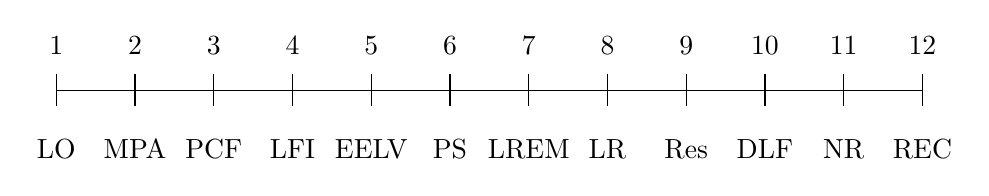
\begin{tikzpicture}
    \draw[-] (1,0) -- (12,0);
    \foreach \x in {1,...,12} {
        \draw (\x,-0.2) -- (\x,0.2);
        \node[below] at (\x,0.8) {$\x$};
	}
    \node[below] at (1,-0.5) {LO};
    \node[below] at (2,-0.5) {MPA};
    \node[below] at (3,-0.5) {PCF};
    \node[below] at (4,-0.5) {LFI};
    \node[below] at (5,-0.5) {EELV};
    \node[below] at (6,-0.5) {PS};
    \node[below] at (7,-0.5) {LREM};
    \node[below] at (8,-0.5) {LR};
    \node[below] at (9,-0.5) {Res};
    \node[below] at (10,-0.5) {DLF};
    \node[below] at (11,-0.5) {NR};
    \node[below] at (12,-0.5) {REC};



\end{tikzpicture}


\caption{M1} \label{fig:M1}
\end{figure}


\end{document}